\chapter{Background and Literature Review}
\section{Forsterite}
The Olivine group of silicate minerals typically contain two end-members: Forsterite, a Mg-silicate, and Faylite, an Fe-silicate, and are abbreviated as Fo and Fa respectively. Naturally occurring olivine is richer in forsterite \citep{johnson2004} in \cite{bearat2006}, for e.g., dunite contains at least $\mathit{Fo_{92}}$ (\SI{92}{\percent} forsterite and \SI{8}{\percent} fayalite by mole) and peridotite typically $\geq\mathit{Fo_{88}}$.
The dissolution reaction of forsterite in a closed system follows the reaction:

\begin{equation}\label{eq:forsterite}
\ce{$\underset{\text{forsterite}}{\ce{Mg_2SiO_4}}$ +  4H^+ -> 2Mg^{+2} + $\underset{\text{dissolved silica}}{\ce{H_4SiO_4}}$}
\end{equation}

Among the many natural occurring silicates, forsterite is an example of a neosilicate. In neosilicates, the silica (\ce{SiO4}) tetrahedra is unpolymerized, i.e., it does not share any oxygen molecules with other silicate tetrahedrons, but instead balances its charge through ionic bonds with interstitial cations like \ce{Mg^{+2}} \citep{olivinebritannica}. This absence of strong interconnecting $\mathrm{Si-O-Si}$ bonds makes it the fastest weathering silicate mineral. The structure of forsterite is illustrated in \Cref{fig:structure}.
\begin{figure}[h]
\centering
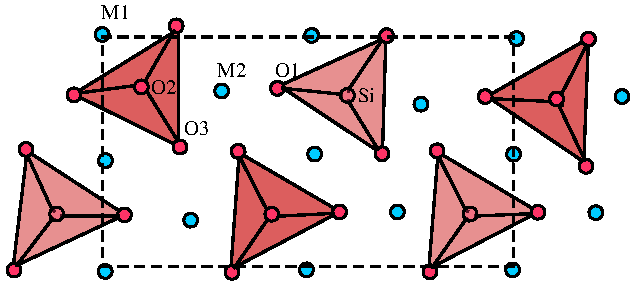
\includegraphics[scale=1]{forsterite.pdf}
\caption{Atomic structure of forsterite with unit cell (marked in black). Oxygen is shown in red, silicon in pink, and Mg in blue.}
\label{fig:structure}
\end{figure}

\section{Enhanced Weathering}
Enhanced weathering (EW) is one of many carbon dioxide removal (CDR) technolgies under the umbrella of climate engineering\footnote{For more information on climate engineering and CDR see \cref{sec:app_ce}}. It aims to accelerate the natural process of weathering by application of powdered minerals over land, ocean, or coastal zones (\citep{schuiling2006,hangx2009} in \cite{renforth2015}). The land application is suitable in warm and humid tropical areas on soil with low pH \citep{schuiling2006,kohler2010}. The suitability of a rock or mineral for EW depends, among other variables, on its reactivity and abundance. Forsterite (Mg-olivine) has one of the highest dissolution rates found in nature \footnote{Carbonates have very high dissolution rates but could be limited in their application due to the high saturation state of dissolved carbonates in oceans. When supersaturated, the `extra' calcium and carbonate ions would precipitate to produce carbonate and release \ce{CO2} back into the atmosphere.} (See \Cref{tab:pH}). Furthermore, rocks like peridotite, basalt, gabbro, and dunite contain the highest concentration of fast weathering silicates, like olivine \citep{hartmann2013}, and constitute around \SI{15}{\percent} of the total land surface area \citep{meybeck1987,hartmann2012}. These factors make forsterite a preferred choice for EW application.

The absorption of \ce{CO2} from the atmosphere in a silicate dissolution reaction is a combination of two reactions. The first reaction is of forsterite with a proton (\ce{H+}), shown in \Cref{eq:forsterite2}. The second is the equilbrium reaction of \ce{CO2} and water (see \Cref{eq:back_eq}). As \ce{H+} is consumed in reaction \ref{eq:forsterite2}, the equilbrium reaction \ref{eq:back_eq}  counteracts this disturbance by absorbing more \ce{CO2} (Le Chatelier's principle) thereby producing more \ce{H+} and \ce{HCO_3^-}. These two reactions are written as a single reaction in \Cref{eq:silicate}. Stochiometrically, $\SI{4}{\mole}$ of \ce{CO2} are absorbed for every $\SI{1}{\mole}$ of forsterite reacted. In terms of mass, $\SI{1}{g}$ of forsterite absorbs $\SI{\sim 1.25}{\gram}$ of \ce{CO2}. 
\begin{equation}\label{eq:forsterite2}
\ce{$\underset{\text{forsterite}}{\ce{Mg_2SiO_4}}$ +  4H^+ -> 2Mg^{+2} + $\underset{\text{dissolved silica}}{\ce{H_4SiO_4}}$}
\end{equation}
\begin{equation}\label{eq:back_eq}
\ce{CO2 + H2O <=> H+ + HCO_3^-}
\end{equation}
\begin{equation}\label{eq:silicate}
\ce{$\underset{\text{forsterite}}{\ce{Mg_2SiO_4}}$ + $\underset{\text{carbonic acid}}{\underbrace{\ce{4H_2O + 4CO_2 (v)}}}$ -> 2Mg^{+2} + 4HCO_3^- +$\underset{\text{dissolved silica}}{\ce{H_4SiO_4}}$
}
\end{equation}
\begin{table}[htbp]
  \centering
    \begin{tabular}{lr}
    \toprule[1.5pt]
    Mineral  & Dissolution Time (years) \\
    \midrule
    Quartz & 34,000,000 \\
    Kaolinite & 6,000,000 \\
    Muscovite & 2,600,000 \\
    Epidote & 923,000 \\
    Microline & 921,000 \\
    Biotite & 900,000 \\
    Albite & 575,000 \\
    Andesine & 80,000 \\
    Bytownite & 40,000 \\
    Enstatite & 10,100 \\
    Diopside & 6,800 \\
    Forsterite & 2,300 \\
    Dolomite & 1.6 \\
    Calcite & 0.1 \\
    \bottomrule[1.5pt]
    \end{tabular}
     \caption{Lifetime of a hypothetical $\SI{1}{mm}$ sphere in a solution at pH 5, in years, for different minerals \citep{lasaga1995}. The minerals listed are various silicates and a few carbonates.} 
 \label{tab:pH}
\end{table}

\section{Calculating the reaction rate}

The reaction rate is defined as the rate of change of concentration of reactants or products. For the dissolution of forsterite (\Cref{eq:forsterite3}), this rate is expressed as \Cref{eq:rate_fo}. $r$ is the extent of reaction and $n_{fo}$ are the moles of forsterite. Further, reactions occurring at the mineral/fluid boundary, also called hetereogenous reactions, are often shown to be dependent on the total or reactive surface area. Hence, the comparison of mineral reaction rates is often done based on rates normalised to surface area (\si{\mole\per\square\metre\per\second}). 
\begin{equation}\label{eq:forsterite3}
\ce{$\underset{\text{forsterite}}{\ce{Mg_2SiO_4}}$ +  4H^+ -> 2Mg^{+2} + $\underset{\text{dissolved silica}}{\ce{H_4SiO_4}}$}
\end{equation} 
\begin{equation}\label{eq:rate_fo}
r=-\frac{dn_{fo}}{dt}=-\textfrac{1}{4}\frac{d[H^+]}{dt}=\textfrac{1}{2}\frac{d[Mg]^{\text{+2}}}{dt}=\frac{d[\ce{H_4SiO_4}]}{dt}
\end{equation}

The rates of chemical reactions, as a function of time or species concentration, are measured in chemical reactors \citep{Brantley2008a}. A batch rector (BR) consists of a tank which is continuously stirred to maintain a homogenous concentration. As the reaction proceeds small samples, called aliquots, of the solution are removed to observe the change in concentration of product, say [Z]. The reaction rate is calculated as follows:
\begin{equation}
\label{eq:back_batch}
r = \frac{1}{A_sm}\frac{dn_Z}{dt}
\end{equation}
where $n_Z$ is moles of element $Z$ in solution, $t$ is time in seconds, $A_s$ is the surface area of mineral in \si{\square\metre}, $m$ is the mass of the mineral in grams. In \Cref{eq:back_batch}, it is assumed that the aliquots are so small that it doesn't influence the total volume of the reactor.

Continuously stirred reactor (CSTR) also called mixed flow reactor (MFR) are flow-through reactors where a mineral is placed in a vessel through which fluid is continuously pumped at flow rate $Q$ \citep{Brantley2008a}. Unlike BR where the the reactor volume can change as aliquots are drawn out over long run, MFR continuously pump liquid in and out of the vessel, such that the volume remains constant. The minerals are suspended in the vessel to maintain ideal mixing. The rate is calculated as:
\begin{equation}
r=\frac{Q([Z_o]-[Z_i])}{A_sm}
\end{equation}

where $Q$ is the flow rate, $[Z_o]$ and $[Z_i]$ are the outlet and inlet concentrations respectively, $A_s$ and $m$ are as before.

A Plug-flow reactor (PFR), also referred as column reactors (when run vertically) or packed-bed reactors are more complex than BR or MFR because of non-ideality of flow and precipitation of products \citep{Brantley2008a}. When the inlet rate is the same as the outflow rate, the rate is calculated as \citep{white2003}:
\begin{equation}\label{eq:back_flow}
r = \frac{Z_o - Z_i}{\beta A_s}\frac{dV}{dt}
\end{equation}

where $Z_i$ and $Z_o$ are inlet and outlet concentrations respectively, $\beta$ is the stochiometric coefficient, $A$ is the mineral surface area, and $dV/dt$ is the rate of flow of fluid through the reactor. Thus, the rate is directly proportional to the product of the (outlet- inlet) concentration and flow rate, and inversely proportional to the surface area. 

\section{Reaction control in mineral dissolution}\label{sec:section2}

In any chemical reaction with multiple steps, the rate of the slowest reaction governs the overall rate of the reaction. The dissolution of minerals occurs through the combination of two distinct processes: the transport of aqueous reactants and products - to and from the surface, and the chemical reactions occurring at the surface \citep{schott2009}. These processes can occur with similar or different rates. If transport of reactants to the surface is faster than the reactions at the surface, the reaction is \textbf{interface/surface- controlled}, or \textbf{transport-controlled} when vice-versa. When their rates are comparable, both processes become important. The terms `controlled' and `limited' have been interchangeably used in the text. 

\subsection{Transport and Surface processes}\label{subsec:transport}
Transport processes can broadly be divided into advection and diffusion. Advection carries away reaction products and transports reactive species from distant regions to the vicinity of the reacting mineral \citep{rimstidt2015}. Advection of a fluid occurs through mechanical agitation, like in a MFR, or when the fluid is subjected to a pressure difference \citep{rimstidt2013}. The latter can also happen due to nonuniform distribution of salinity and temperature. Diffusion, on the other hand, is driven by concentration gradients across --- a fluid boundary layer (the thin layer of immobile fluid in contact with the mineral surface) \citep{rimstidt2015}, an alteration layer/leached layer on the mineral surface \citep{luce1972,Brantley2008b}, solid-state diffusion \citep{luce1972}, or a combination of the three.
\noindent The transport rate is measured as a transport flux with units of \si{\mole\per\square\metre\per\second}.

Surface processes refer to the basic molecular steps leading to detachment of a cation or other atom from the mineral bulk into the bulk solution \citep{Brantley2008c}. These processes depend on the physical and chemical properties of the mineral (also called intrinsic factors) \citep{white2002}, for e.g., molecular composition, reactive surface area etc.; they are discussed in detail in \Cref{sec:rate_control}. 

\section{Characteristics of Forsterite dissolution}\label{sec:rate_control}

\subsection{Nonstochiometry}\label{subsec:nonstochio}
A reaction is stochiometric and shows congruent dissolution when the consumption of reactants and release of products follow the reaction stochiometry. For \cref{eq:forsterite3}, this would mean that 1 mol of forsterite dissolves completely to produce 2 moles of \ce{Mg^{+2}} and \SI{1}{\mol} of dissolved silica (\ce{H_4SiO_4}). However, many silicates show nonstochiometry and thus incongruent dissolution. This behaviour can be due to dissolution of impurities within the mineral, by precipitation of secondary minerals, or by preferential leaching of elements from the mineral surface \citep{Brantley2008b}. Past experiments on forsterite dissolution have observed nonstochiometry in the initial phase of the dissolution (becoming stochiometric after a few hundred hours of reaction); that has been attributed to to the formation of a Si-rich amorphous layer on the mineral surface \citep{wogelius1992,pokrovsky2000,hellmann2012}. Nonstochiometry is more pronounced at lower pH. At steady state, the thickness of this layer has been reported to be around \SIrange[range-units = single,range-phrase = --]{1}{5}{\nano\meter} \citep{pokrovsky2000,hellmann2012} at \SI{25}{\degreeCelsius}.

Until recently, the formation of the Si-rich layer was believed to be due to the preferential leaching of Mg compared to Si \citep{luce1972,paces1973,pokrovsky2000,lee2008}  followed by the slow hydrolysis and subsequent leaching/release of the Si and O into the bulk solution. This resulted in the formation of an outer layer, rich in Si or depleted in Mg, called leached or depleted layer after the mechanism involved. \cite{hellmann2012}, however, using high-resolution images showed that both Mg and Si dissolve congruently into the solution irrespective of the pH and involve no preferential leaching. Only Si reprecipitates back on the surface leading to formation of the Si-rich layer. This theory of dissolution-reprecipitation calls the Si-rich layer simply as a surface layer. The mechanism and terminology from \cite{hellmann2012} will be used in the text.

\subsection{Non steady state}\label{subsec:nonsteadystate}
The first experiments on forsterite dissolution in mixed-flow reactors observed the reaction rate to decrease with time as a power function of the form $r=kt^{\text{0.5}}$\;\citep{luce1972,paces1973}, giving rise to the term \textit{parabolic kinetics} \citep{Brantley2008b}. This non-steady state behavior is attributed to the initial fast dissolution of fine particles and surface sites with high energy (created during the crushing and grinding of a mineral), as well as non-stochiometric dissolution (\cite{holdren1979} in \cite{Brantley2008b}). However, cleaning of the initial material to remove fines and using a low rock to fluid volume ratio result in apparent steady state rates in a few hundred hours and thus provide a means of comparison across experiments. 

\subsection{Factors affecting rate of dissolution }\label{subsec:factors}
The following section summarises the most up-to-date knowledge on factors affecting rate of forsterite dissolution, particularly at ambient temperatures and above neutral to alkaline pH range, and the conceptual or experimental problems associated with their measurement.  
\subsubsection{Effect of pH and temperature}
The effect of pH and temperature on rate of forsterite dissolution has been rigorously studied \citep{wogelius1991,wogelius1992,pokrovsky2000,rosso2000,oelkers2001a}
The effect of the main factors on the rate has been summarised by \cite{rimstidt2012} into a rate equation (normalised to BET surface area):
\begin{subequations}\label{eq:rimstidt}
\begin{equation}
\mathrm{log\;Rate_{BET} = 5.17-0.44pH-3675/T \qquad \text{for pH < 5.6}}
\end{equation}
\begin{equation}
\mathrm{log\;Rate_{BET} = 2.34-0.22pH-3179/T \qquad \text{for pH > 5.6}}
\end{equation}
\end{subequations}

\Cref{eq:rimstidt} show that the reaction rate is directly proportional to the pH, or [\ce{H+}], and the Temperature. 
\subsubsection{Effect of partice size and surface area}\label{subsec:sa_sec}
Along with temperature and pH, the surface area is the most important factor controlling reaction rate \citep{rimstidt2012}. However, unlike pH and temperature, it has not been rigorously studied for forsterite. 

Comparison of reaction rates (at similar conditions) from past studies reveals large errors (\num{\sim 0.5} log units) when normalised to geometric surface area \citep{rimstidt2012}. These errors were attributed to experimental and conceptual problems. The experimental problems concern with factors affecting BET measurement--- preparation of sample, pre-treatment of sample, mineral composition and adsorbent gas used\;\citep{brantley2000,rimstidt2012,rosso2000}. Even though BET measurements of a same sample on the same machine are highly reproducible (error of \SI{\pm 5}{\percent} \citep{brantley2000}), the factors mentioned above become important when measurements are compared across laboratories. 

A mineral surface is composed of sites with different surface energies and the reactivity of a mineral is controlled by the number and distribution of these sites, and the crystallographic axes	\citep{grandstaff1978,awad2000,Brantley2008c}. These constitute the reactive \citep{white1990} or the effective surface area \citep{aagaard1982,helgeson1984}. However, most studies on finding dissolution rates don't use them; instead, the total surface area (TSA) (also known as the BET surface area), or the geometric surface area is used \citep{Brantley2008c}. This assumption implies that reacting sites are homogeneously distributed and all surface sites are equally reactive\; \citep{grandstaff1978,white1990}. Moreover, the relation between surface area and reaction rate is assumed to be the same across all grain sizes \citep{grandstaff1978}. \cite{holdren1987} experimenting with feldspars, show that this assumption breaks down for particles \SI{<75}{\micro\meter} and that for particles in this region no clear relation exists between rate and surface area. This result is also supported by experiments of \cite{kleiv2006}.

Lastly, reaction rates are often normalised to initial surface area (geometric or BET) but the reaction at any moment depends on the reactive surface area available at a particular point of time. 

The above mentioned points highlight the experimental problems and conceptual assumptions associated with surface area. These must be considered on any discussion or comparison of reaction rates.
\subsubsection{Effect of reaction products and other ions}
The effect of reaction products (see \cref{eq:forsterite}) on reaction rate have been explored by a few studies. \cite{oelkers2001a} observe that forsterite dissolution rates are unaffected by aqueous Mg and Si at pH 2, whereas \cite{pokrovsky2000} show that the rate decreases at pH 9 and 11 as a function of Si concentration. Both experiments were carried in MFRs at \SI{25}{\degreeCelsius}. \cite{rimstidt2012} summarise that water activity (\num{>0.9}), [\ce{SO_4^{2-}}] \SI{>3}{M}, and Ionic Strength \SI{<12}{M} do not significantly affect rates.
\subsubsection{Effect of \ce{CO2} and carbonates}
Even though most laboratory experiments on forsterite dissolution were held in closed systems and took into account only hydrolysis of forsterite, real world application --- for calculating natural \ce{CO2} consumption through weathering, enhanced weathering, or mineral carbonation require the interaction of the basic hydrolysis reaction with \ce{CO2} or dissolved carbonate ions. These could influence rate directly - by formation of surface complexes during interaction, or indirectly - by control of pH \citep{awad2000}. The overall effect of dissolved \ce{CO2} on forsterite dissolution isn't understood because of contradictory results. \cite{golubev2005} reported that there is no effect of p\ce{CO2} (p is partial pressure) on the rate of dissolution, while \cite{wogelius1991} reported a decrease in the rate of dissolution of olivine. Further, the effect of p\ce{CO2} might be dependent on the pH and that it might be important in alkaline conditions \citep{hanchen2006,wogelius1991}. According to \cite{rimstidt2012} existing data set is not sufficient to quantify any affect of dissolved carbonates, and even under alkaline conditions at constant pH, silicate dissolution rates show only a negligible or at best weak dependence on p\ce{CO2} \citep{Brantley2008c}. 

\begin{figure}[h]\label{fig:rate_control}
\centering
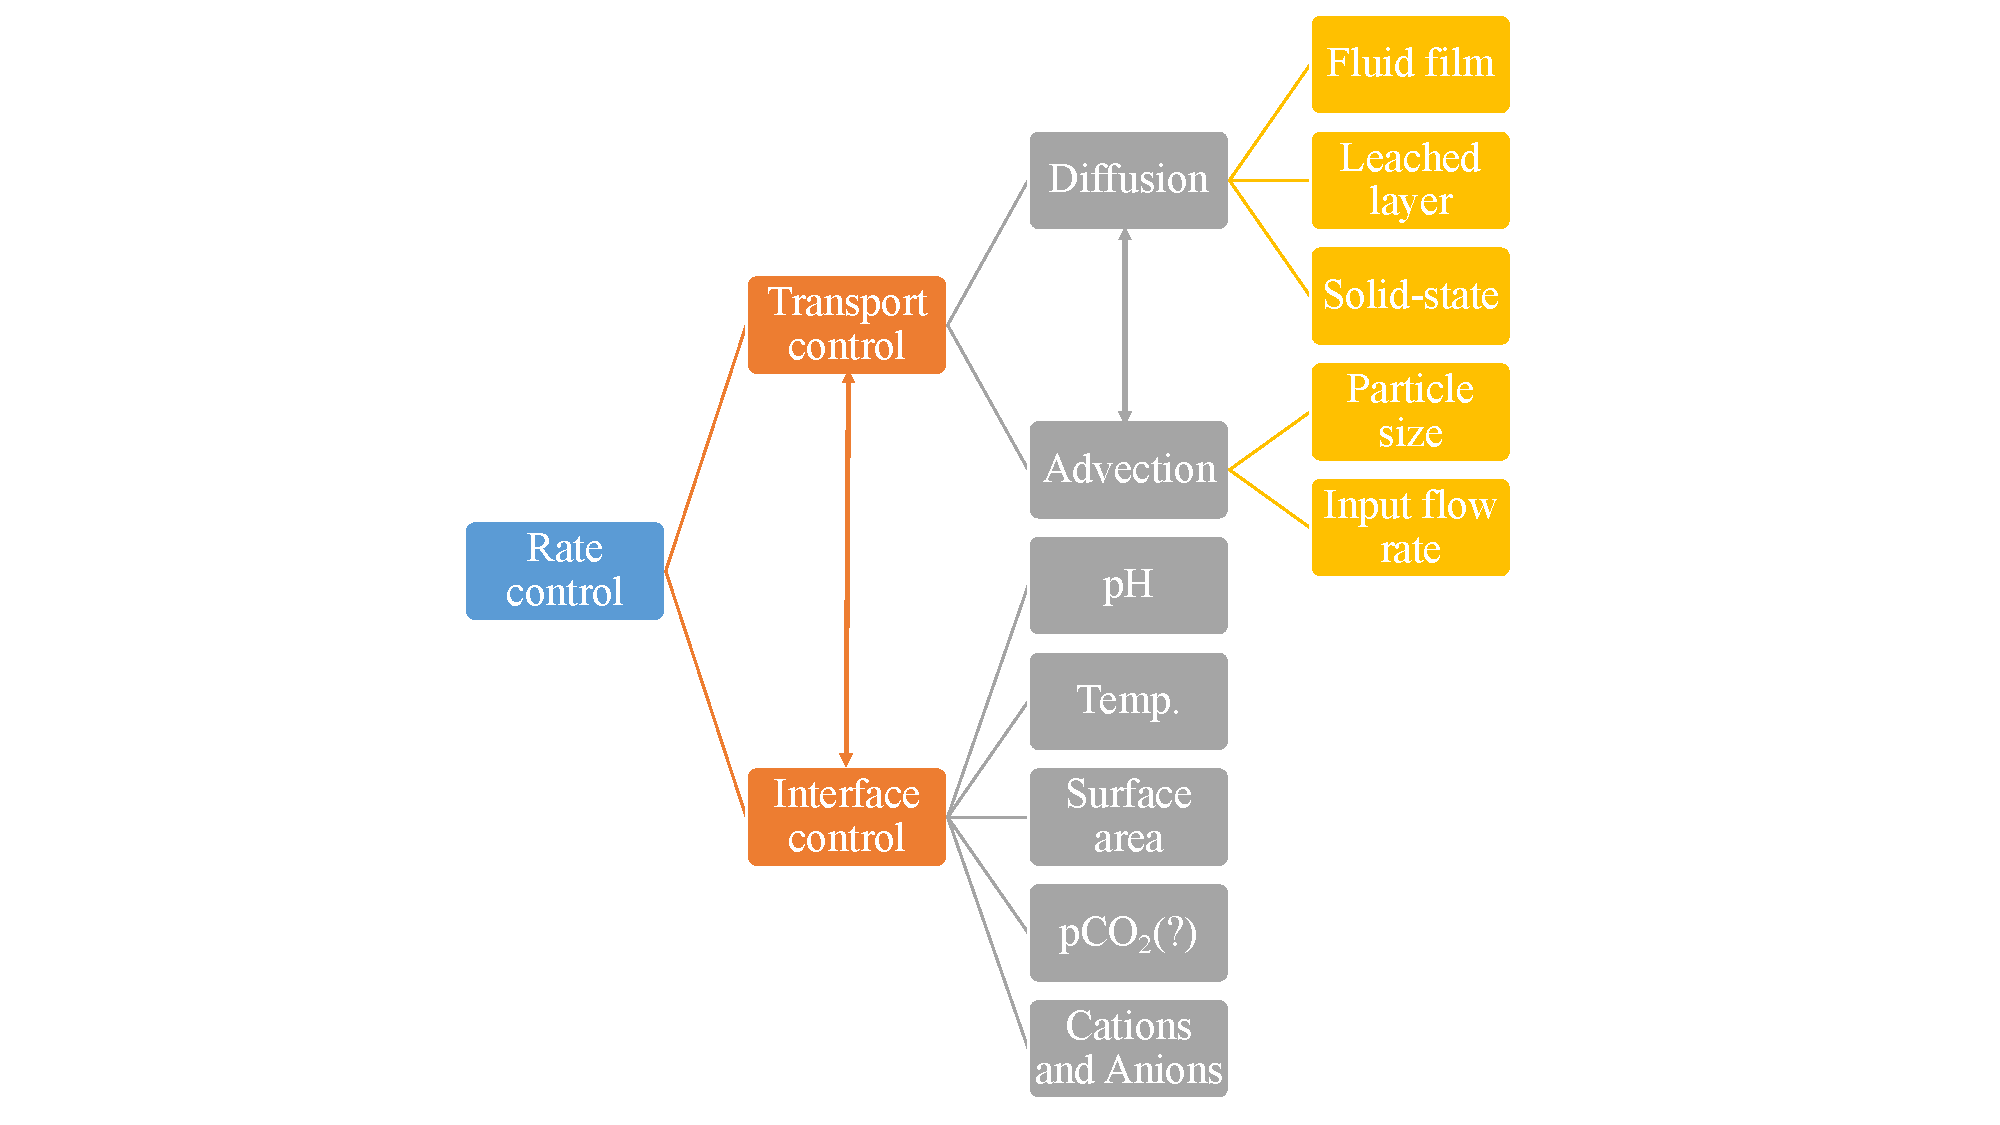
\includegraphics[scale=0.5]{rate_control.pdf}
\caption{Factors affecting rate control in silicate dissolution. The double sided arrows represent the possibility when both processes become important or influence each other. The surface processes are taken for forsterite but the transport processes are generic. }
\end{figure}
 
\subsection{Rate control in forsterite dissolution}
Results from previous studies point toward the dissolution of forsterite being surface limited. According to \cite{schott2009}, for most rock-forming minerals\footnote{Forsterite is also a rock-forming mineral} at ambient temperatures, chemical reactions at the solid interface are slow and thus rate limiting. \cite{wogelius1991,brady1989} show that the control of dissolution reactions for silicates clearly occurs at the surface. To test for transport control in laboratory experiments \cite{luce1972} changed the agitator speed of the reactor but found no change in the reaction rate, implying surface control. The concept of reaction control can also be understood in terms of energy requirements --- at low temperatures the activation energy of the of the mineral interface (\SI{\sim 15}{kcal\per\mole}) is often higher than that of diffusion (\SI{\sim 5}{kcal\per\mole}) \citep{Brantley2008b}. Perhaps for the same reasons mentioned above, \cite{rimstidt2012}, in their compilation of past studies assume rate to be interface limited for all experiments even though there was insufficient information in the literature to quantify the hydrodynamics \citep{rimstidt2012}. However, most laboratory experiments on forsterite dissolution have been carried out at small rock to volume ratios, i.e., a few grams or milligrams of the mineral are taken in comparatively large batch and mixed-flow reactors \citep{awad2000,martinez2014} and thus might not have been susceptible to transport control. Among various reactor designs, Plug-Flow Reactors (PFRs) with packed-beds (also called packed-bed reactors) are highly susceptible to be transport-controlled and also better mimic natural systems \citep{Brantley2008a}, but few experiments with packed beds exist for forsterite. For e.g., in the compilation of past forsterite dissolution studies \citep{rimstidt2012} only one experiment, that of \cite{kleiv2006}, was performed in a PFR. More recently, \cite{renforth2015}, conducted packed-bed experiments on a mixture of olivine and soil. An illustrative flow-chart on the factors affecting rate-control in forsterite is shown in \Cref{fig:rate_control}.

As discussed in \cref{subsec:transport}, the diffusion of reactants or products between the bulk-solution and the mineral surface occurs across a layer/region. This layer could be the immobile fluid boundary layer, leached/altered layer, or the solid itself. \cite{hellmann2012} argue that 
both the Si-rich layer formed on forsterite or solid-state diffusion are not rate controlling, mainly because of the small thickness and high porosity of the altered layer.  \cite{rimstidt2015} through modeling studies for a packed bed/column of forsterite and assuming diffusion of \ce{H+} through a fluid film show that under certain conditions rate can become transport-limited. This model will be used and discussed in detail later. 

\section{Motivation}
The application of olivine or other silicate containing rock for EW can be imagined as spreading of rock powder on, for e.g., agricultural farms resulting in a layer/column of the material. The current study aims to find the kinetics of olivine dissolution in column experiments and to understand the variables affecting it.  
 